\subsection{Quench detection}
{{\footnotesize
\noindent Exploration of real-time quench detection using unsupervised and RL approaches, combining multi-modal sensor data (BPM, power supply, acoustic), operating on kHz-MHz streams with anomaly detection and frequency-domain features.


\begin{description}[labelwidth=4cm, labelsep=1em, leftmargin=4cm, itemsep=0.1em, parsep=0em]
  \item[date:] 2024-10-15
  \item[version:] v1.0
  \item[last\_updated:] 2024-10
  \item[expired:] no
  \item[valid:] yes
  \item[valid\_date:] 2024-10-15
  \item[url:] \href{https://indico.cern.ch/event/1387540/contributions/6153618/attachments/2948441/5182077/fast\_ml\_magnets\_2024\_final.pdf}{https://indico.cern.ch/event/1387540/contributions/6153618/attachments/2948441/5182077/fast\_ml\_magnets\_2024\_final.pdf}
  \item[doi:] NA
  \item[domain:] Accelerators and Magnets
  \item[focus:] Real-time detection of superconducting magnet quenches using ML
  \item[keywords:]
    - quench detection
    - autoencoder
    - anomaly detection
    - real-time
  \item[licensing:] Via Fermilab
  \item[task\_types:]
    - Anomaly detection
    - Quench localization
  \item[ai\_capability\_measured:]
    - Real-time anomaly detection with multi-modal sensors
  \item[metrics:]
    - ROC-AUC
    - Detection latency
  \item[models:]
    - Autoencoder
    - RL agents (in development)
  \item[ml\_motif:]
    - Real-time, RL
  \item[type:] Benchmark
  \item[ml\_task:]
    - Reinforcement, Unsupervised Learning
  \item[solutions:] 0
  \item[notes:] Precursor detection in progress; multi-modal and dynamic weighting methods

  \item[contact.name:] Maira Khan
  \item[contact.email:] unknown
  \item[datasets.links.name:] BPM and power supply data from BNL
  \item[results.links.name:] ChatGPT LLM
  \item[fair.reproducible:] in progress
  \item[fair.benchmark\_ready:] False
  \item[id:] quench\_detection
  \item[Citations:] \cite{quench2024}
\end{description}

{\bf Ratings:} ~ \\

\begin{tabular}{p{0.15\textwidth} p{0.07\textwidth} p{0.7\textwidth}}
\hline
Rating & Value & Reason \\
\hline
dataset & 2 & Dataset URL is missing; FAIR principles largely unmet
 \\
documentation & 2 & Only a conference slide deck is available; lacks detailed instructions or repository for reproduction
 \\
metrics & 3 & ROC-AUC and latency are mentioned, but metric definitions and formal evaluation setup are missing
 \\
reference\_solution & 1 & No baseline or reproducible model implementation available
 \\
software & 1 & Code not provided; no evidence of documentation or containerization
 \\
specification & 4 & Real-time detection task is clearly described, but exact constraints, inputs/outputs, and evaluation protocol are only partially specified
 \\
\hline
\end{tabular}

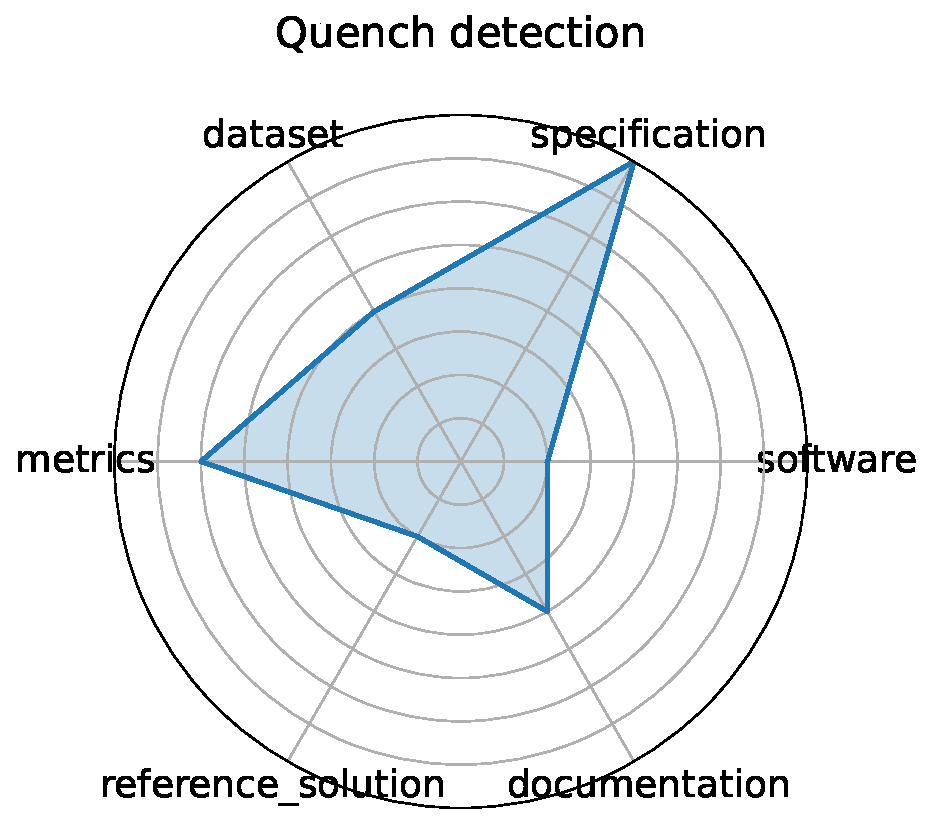
\includegraphics[width=0.2\textwidth]{quench_detection_radar.pdf}
}}
\clearpage